\section{Patron de reconfiguration}

\begin{frame}{Réutilisation des décisions de reconfiguration}
Critères de réutilisation
\begin{itemize}
\item \textbf{Titre} : méthaphore                                                                   
\item \textbf{Intention} : description générale                                                                   
\item \textbf{Contexte} : hypothèse de la solution                                                                    
\item \textbf{Problème} : besoins à satisfaire                                                                     
\item \textbf{Solution} : résolution du problème                                                                     
\item \textbf{Conséquence} : description effets sur les aspects non
fonctionnels                                                              
\end{itemize} 
\end{frame}


\begin{frame}[fragile]{Type de documentation des décisions : docu.
formelle \emph{Allen, 1998}}
\centering
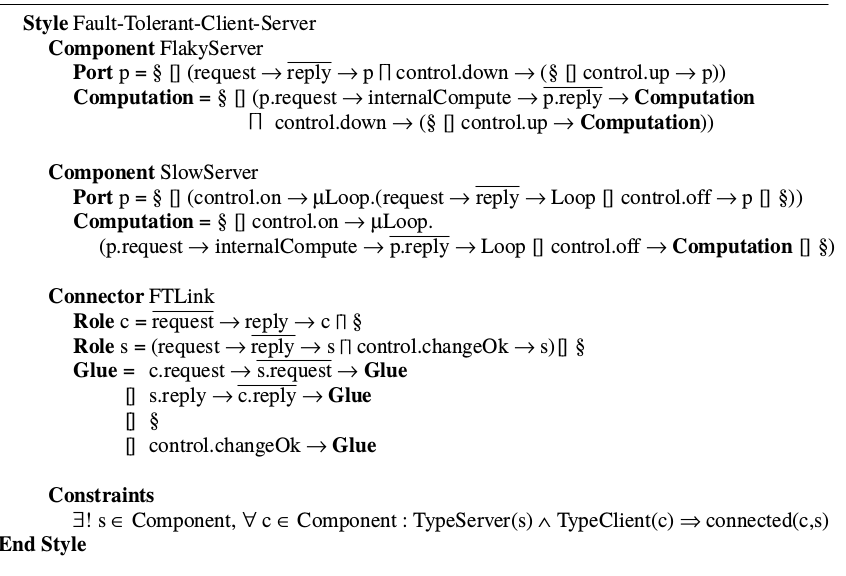
\includegraphics[width=5cm]{imgs/slide_fault-tolerance.png}
\hspace{1cm}
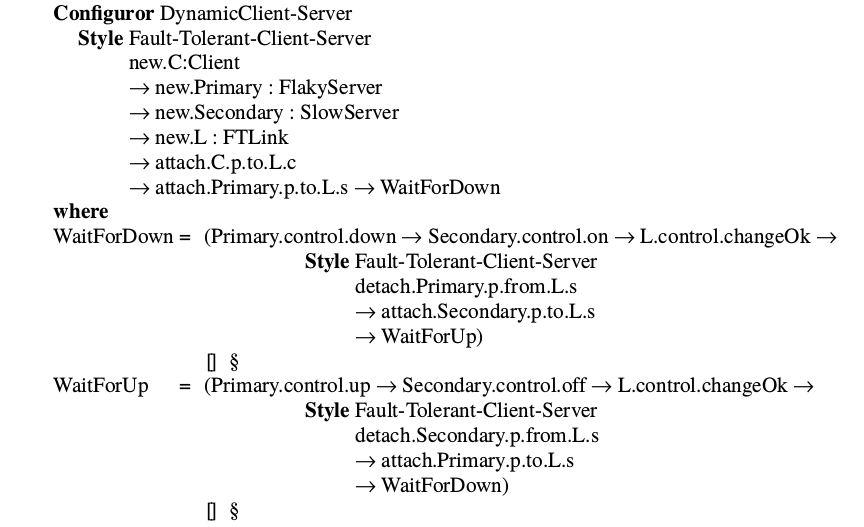
\includegraphics[width=5cm]{imgs/slide_reconf_specif.png}
\vspace{0.5cm}
\begin{table}[]
\resizebox{0.85\textwidth}{!}{%
\begin{tabular}{ccccccc}
         & Titre     & Intention & Contexte  & Problème  & Solution  & Conséquence \\
Allen    & \ding{53} & \ding{53} & \ding{51} & \ding{51} & \ding{51} & \ding{53}   \\
\end{tabular}}
\end{table}
\end{frame}

%\captionsetup[subfigure]{labelformat=empty}
\begin{frame}[fragile]{Type de documentation des décisions : docu. formelle
\emph{Oliveira, 2015}}
\centering

\includegraphics[width=8cm]{imgs/slide_oliveira_primitive.png}\\
\textbf{Contexte : primitive de reconfiguration}\\
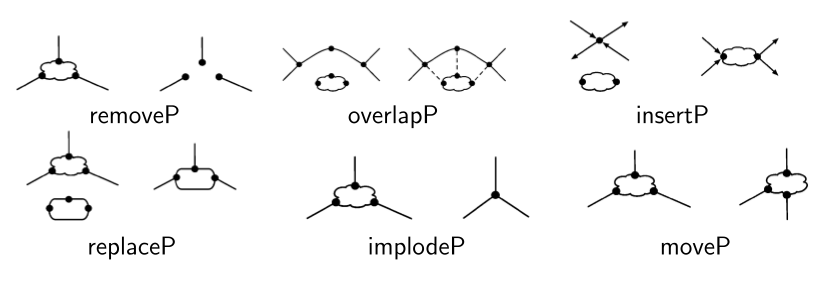
\includegraphics[width=8cm]{imgs/slide_oliveira_patron.png}\\
\textbf{Patron de reconfiguration}
\begin{table}[]


\resizebox{0.85\textwidth}{!}{%
\begin{tabular}{ccccccc}
         & Titre     & Intention & Contexte  & Problème  & Solution  & Conséquence \\
Oliveira & \ding{51} & \ding{53} & \ding{51} & \ding{53} & \ding{53} & \ding{53}
\end{tabular}}
\end{table}
\end{frame}

\begin{frame}[fragile]{Type de documentation des décisions : docu.
semi-formelle
\emph{Gomaa, 2004}}
Titre : Master-Slave Reconfiguration Pattern, Centralized Control
Reconfiguration Pattern, Client / Server Reconfiguration Pattern,
Decentralized Control Reconfiguration
Pattern.
\begin{figure}
\begin{subfigure}[b]{0.5\textwidth} % "0.45" donne ici la largeur
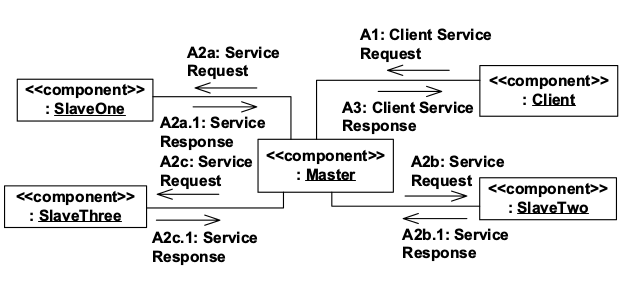
\includegraphics[width=3cm]{imgs/gomaa_contexte}
\caption{Contexte}\label{fig:orchid}
\end{subfigure}
\begin{subfigure}[b]{0.5\textwidth} % "0.45" donne ici la largeur
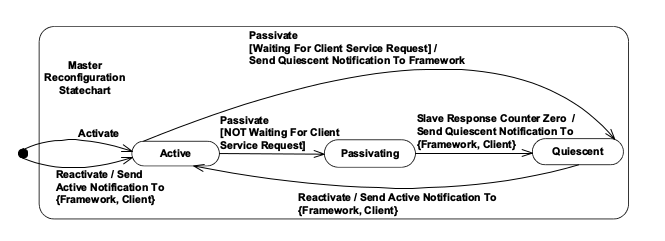
\includegraphics[width=3cm]{imgs/gomaa_solution}\\
\caption{Solution}\label{fig:orchid}
\end{subfigure}
\end{figure}
\end{frame}

\begin{frame}{Résumé caractéristique des décisions de reconfiguration
pour les SdSs}
\begin{table}[]
\centering
\resizebox{0.85\textwidth}{!}{%
\begin{tabular*}{\textwidth}{c @{\extracolsep{\fill}} ccccccc}
%\begin{tabular}{cccccccc}
         & Titre     & Intention & Contexte  & Problème  & Solution  & Conséquence \\
Allen    & \ding{53} & \ding{53} & \ding{51} & \ding{51} & \ding{51} & \ding{53}   \\
Oliveira & \ding{51} & \ding{53} & \ding{51} & \ding{53} & \ding{53} & \ding{53}   \\
Gomaa    & \ding{51} & partielle & partielle & \ding{51} &\ding{51}  & \ding{51}   
\end{tabular*}
}
\end{table}
\end{frame}


\begin{frame}{Patron de reconfiguration : délimitation du problème}
\begin{figure}
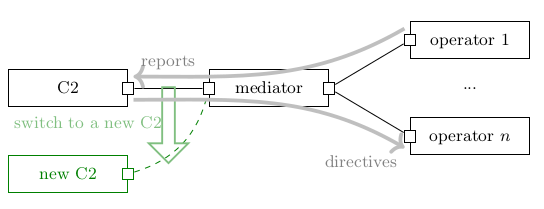
\includegraphics[width=8cm]{imgs/dc_archi-C2}
\end{figure}

Invariants :
\begin{itemize}
\item Pendant la
reconfiguration, les deux C2 partagent le même état de mission.
\item Pendant la
reconfiguration, tous les opérateurs sont connectés à exactement un
C2. 
\end{itemize}

Forces :
\begin{itemize}
\item instancier une deuxième version du composant qui coexiste avec
la version initiale; et
\item synchroniser les états partagés entre les versions du
composant.
\end{itemize}

\end{frame}

\begin{frame}{Patron de reconfiguration : description de la solution}
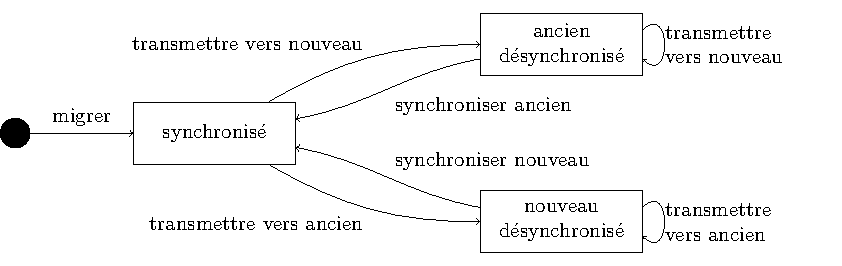
\includegraphics[width=12cm]{imgs/slide_solution_coevolution.pdf}
\end{frame}

\begin{frame}{Résumé}
\begin{itemize}
\item Quiescence : dont l'objectif le principe est de rendre passif,
les composants dépendant du composant ciblé par la reconfiguration. 
\item Tranquilité : est une variante de la quiescence qui assouplie
les critères de reconfiguration. Elle décrit les conditions dans
lesquelles la reconfiguration pêtre réalisée sans attendre l'état de
tranquilité
\item Co-evolution : contrairement à la quiescence et tranquilité, à
déployer directement la nouvelle version du composant ciblé par la
reconfiguration. La conséquence est que les deux versions d'un
composant s'execute simultanément. 
\item Opportuniste : par rapport aux autres, il concerne une
granularité différente puisqu'il concerne seulement une opération de
déconnexion et connexion qui est réalisé dès que l'occasion se
présente.  
\end{itemize}
\end{frame}
